\chapter{Background}
The problem space we explore ties together work across a number of different disciplines, including graphics, graphic design, and machine learning modeling.
In hoping to apply generative methods to vectorized glyphs, we are inspired by previous work in computer vision on non-natural images and draw upon recent developments in generative modeling of line drawings.

\section{Non-natural images}
While natural images are photographs of real-world scenes and objects, non-natural images are computationally generated, either by hand with a computer design tool or automatically.
Images in this category include graphs, pictograms, virtual scenes, graphic designs, and more.
Algorithmically understanding, summarizing, and synthesizing these images pose unique challenges because of the images' clean and deliberately drawn designs, sometimes multimodal nature, and human-imbued intent. 

While much attention has been focused on research problems like object recognition, scene segmentation, and image recognition on natural images, interest in applying computer vision methods to non-natural images has been growing.
Much progress has been made towards computationally understanding non-natural images on datasets including XML-encoded scenes~\cite{wu2017neural}, comic strips~\cite{iyyer2016amazing}, and textbook diagrams~\cite{seo2014diagram}.
Recent work by our group has explored the space of infographics, complex diagrams composed of visual and textual elements that deliver a message~\cite{bylinskii2017understanding}.

\subsection{Font faces}
Within the space of non-natural images, we focus specifically on designer-crafted font faces.
Fonts are used to typeset text with particular styles and weights, and many types of fonts exist, including serif, sans serif, and handwriting style fonts.
Each font is defined by a set of glyphs, which include letters, digits, symbols, and potentially other Unicode characters.
Within a font face, glyphs generally share the same style for properties like angles, curvature, presence of serifs, and stroke width.

In the context of computational modeling and generation, font glyphs offer certain advantages and pose distinctive challenges when compared to other types of designed graphics.
Unlike more complicated designs such as infographics and diagrams, they can essentially be represented as drawings composed of simple lines and curves and, as such, can be modeled using sequential drawing commands.
However, font glyphs have distinct classes (i.e.\ each letter, number, symbol, etc.\ is a different class) and thus designing a generation procedure that is able to create clearly defined instances of different classes presents a difficult problem.

In this work, our computational methods are applied to font faces downloaded from Google Fonts\footnote{Downloaded from \url{https://github.com/google/fonts}, a GitHub repository containing all fonts in the dataset.}.
In Figure~\ref{fig:input_fonts}, a sampling of glyphs from the Google Fonts dataset is shown.

\begin{figure}[]
	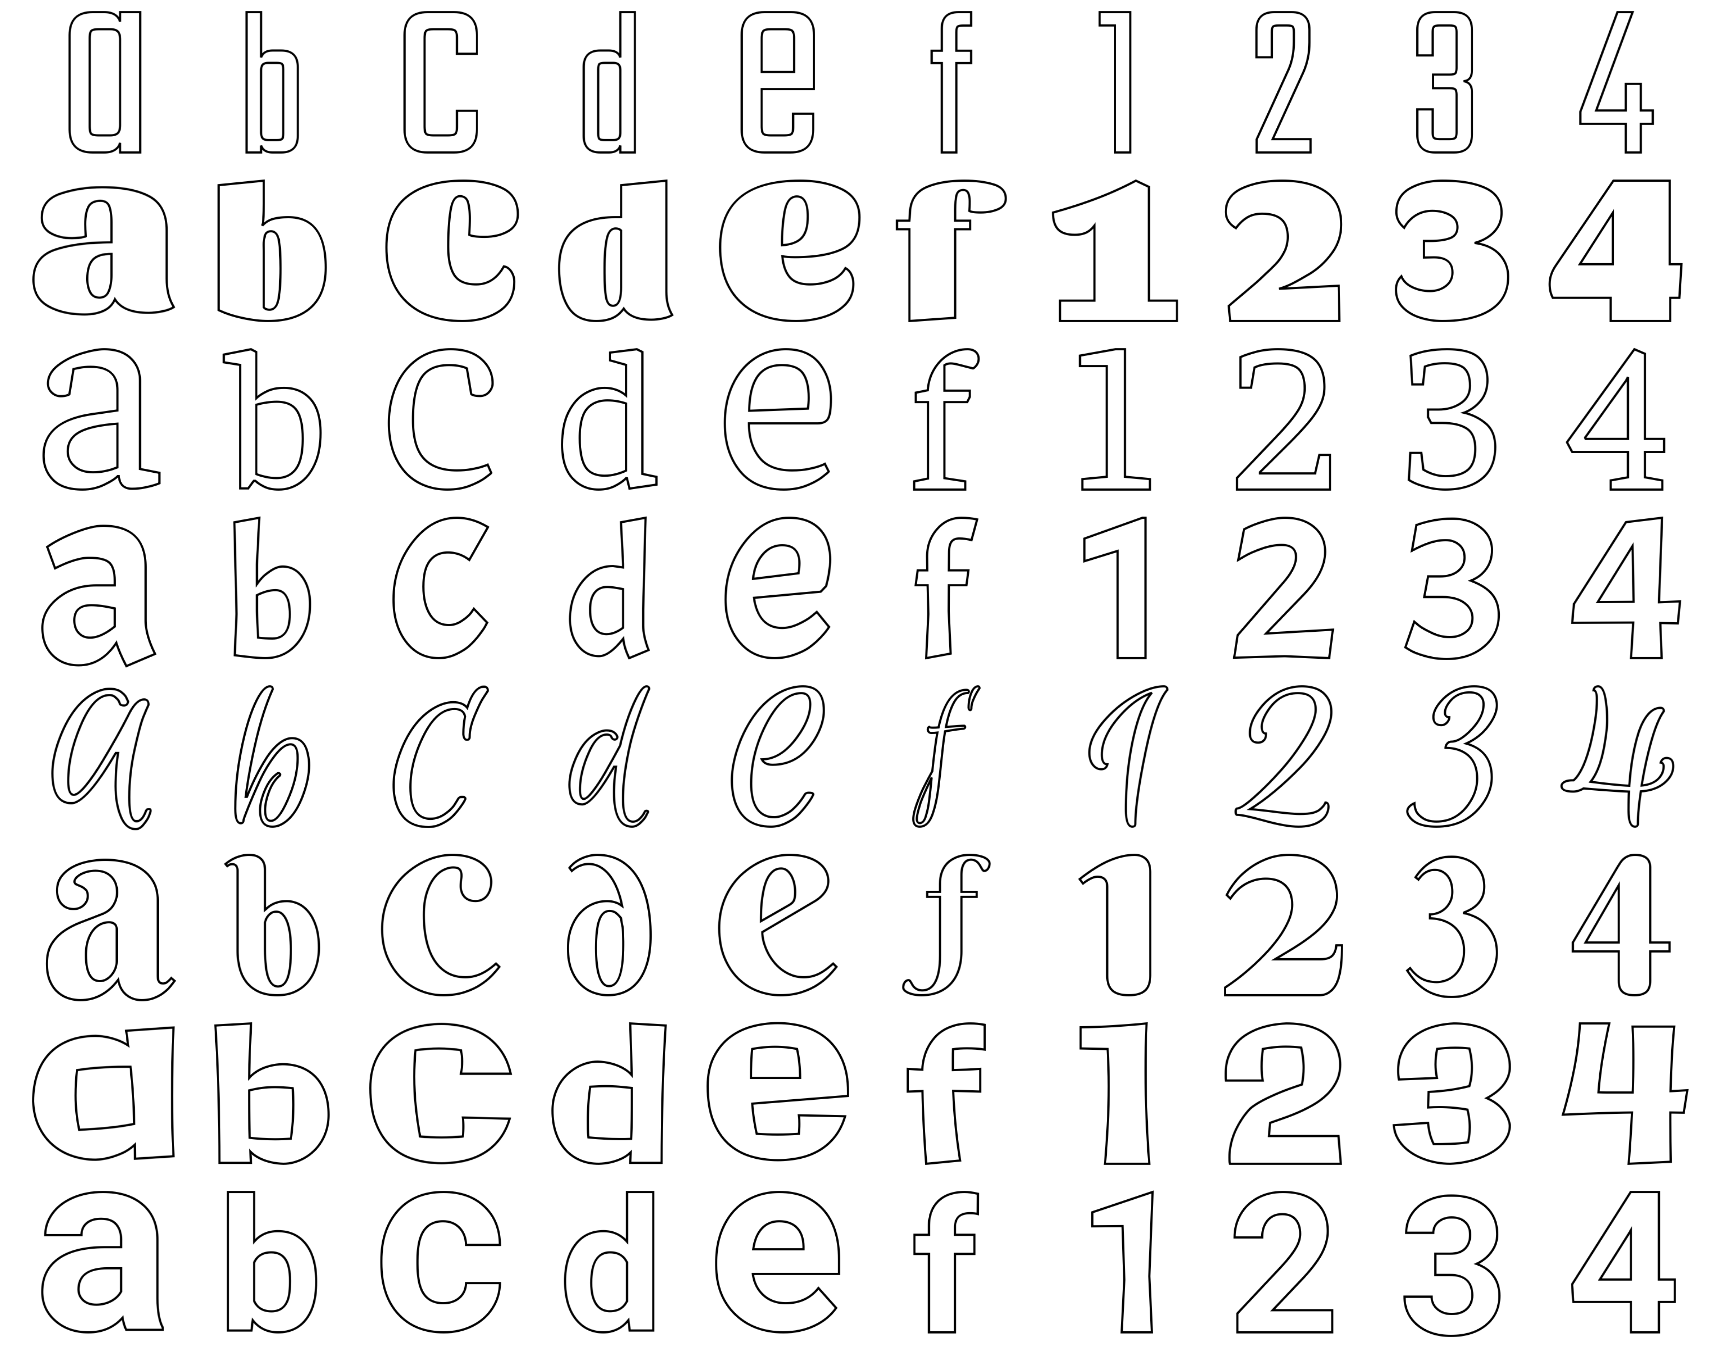
\includegraphics[width=\textwidth]{figures/input_fonts}
    \caption[A sample of the types of font faces used in our fonts dataset]{A sample of the types of font glyphs used in our dataset. Lowercase letters ``a'' through ``f'' are shown, as well as digits 1 through 4. Note the variety of styles represented: the dataset includes serif, sans serif, display, and handwriting style fonts.\label{fig:input_fonts}}
\end{figure}

\subsection{Vector graphics}
We are primarily interested in applying computational models to vector graphics as opposed to raster images.
While raster images encode color values for each point (or \textit{pixel}) in a two-dimensional grid, vector graphics describe a set of curves and shapes parameterized by mathematical equations and control points.
Many specifications exist for describing images in vector format, including SVG, Encapsulated PostScript (EPS), and Adobe PDF\@.
Font faces are often distributed as TrueType (TTF) files, which encode line and curve commands as well as font hints to aid with rendering.

Although the focus of our research is on font glyph inputs, our vision is to build a generalizable system for the variety of vector graphics generated by designers.
Thus, our system accepts SVG data as input, as most vector graphics formats (including TTF) can be expressed using the commands available in the SVG specification.

\begin{figure}[t]
    \subcaptionbox{Raster images are defined as two-dimensional arrays of pixel values, while vector graphics define curves and paths mathematically. Thus, when scaled, vector graphics (right) can still be rendered smoothly while raster images (left) degrade in quality.\label{fig:svg-a}}
    {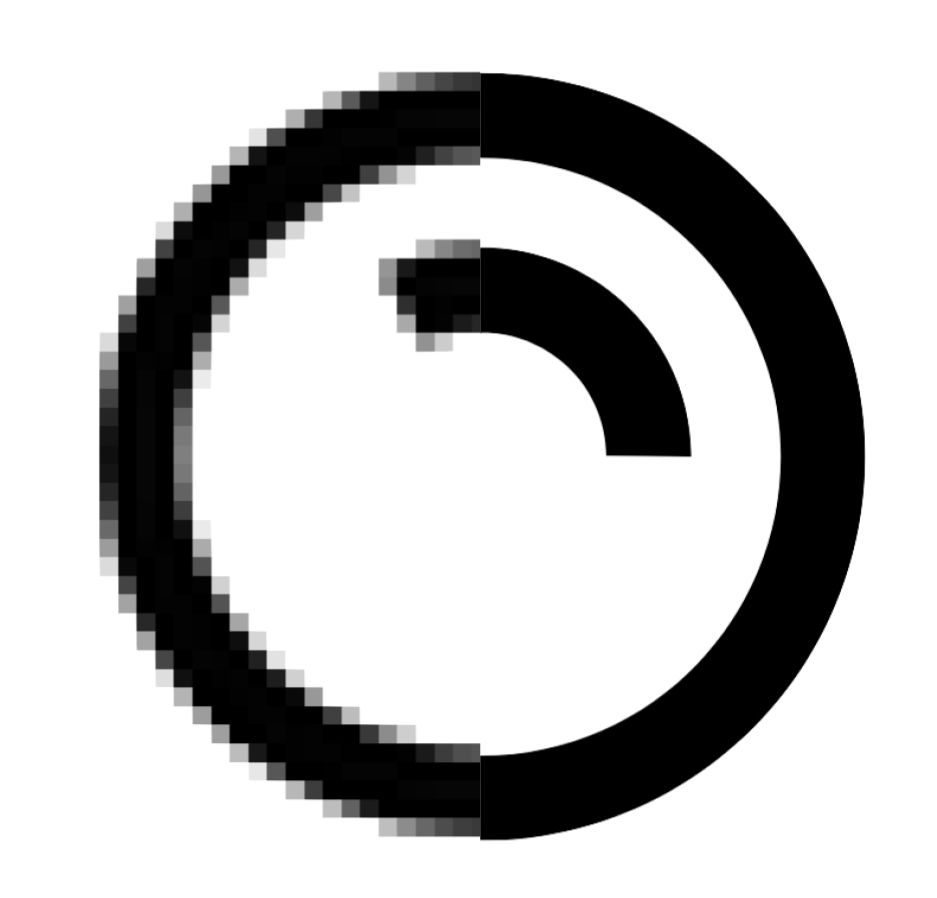
\includegraphics[height=1.85in]{figures/b_vs_vec}} \quad
    \subcaptionbox{SVG is an XML-based markup language that describes geometric elements within a vector image. A single path is used to draw this soap bubble, and colored curves in the image correspond approximately to the highlighted attribute commands that describe them. For example, the command \code{l-0.69-1.32} indicates a line drawn from a starting point to a point 0.69 units to the left and 1.32 units down.\label{fig:svg-b}}
    {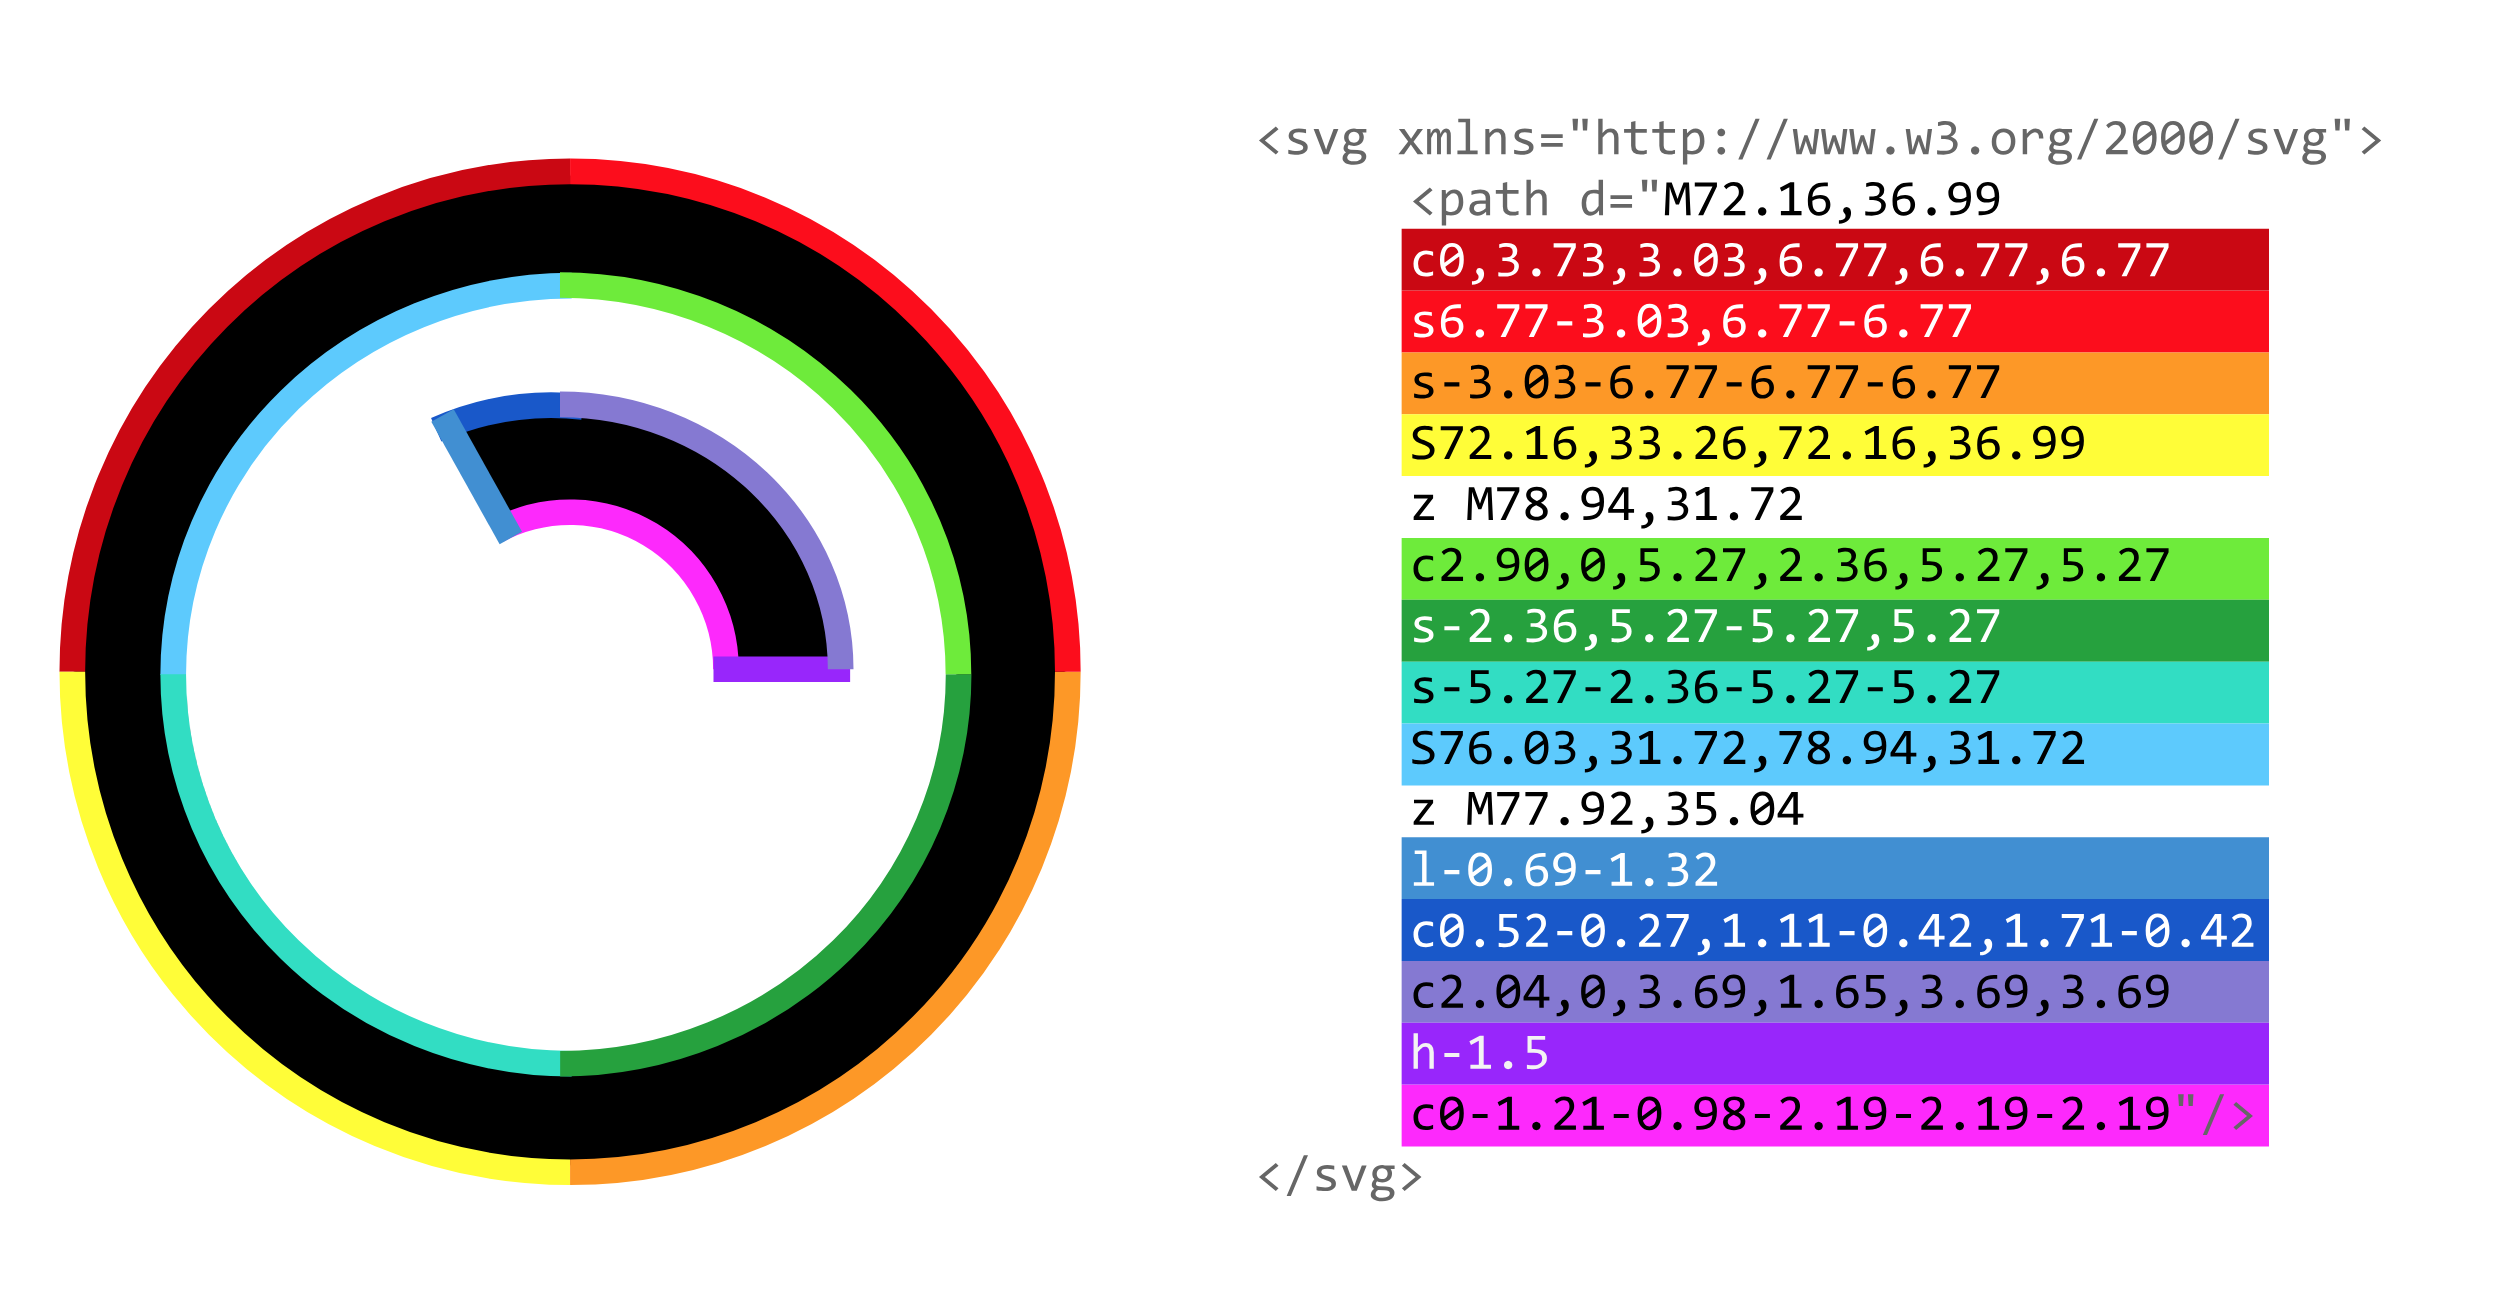
\includegraphics[height=1.85in]{figures/svgs}}
    \caption[An overview of the specification for scalable vector graphics (SVG)]{a visual comparison of raster and vector graphics. Figure~\ref{fig:svg-b} walks through a sample vector graphics path. Image source: \textit{Dog Wash} by Llisole from the Noun Project.\label{fig:svg}}
\end{figure}

\subsubsection{Modeling vector graphics}
Applying computer vision techniques to vector graphics raises new challenges.
While bitmap and vector data can both decode into the same visual output, their underlying encoding structures have vast differences (Figure~\ref{fig:svg-a}).
As a data format, SVGs describe lists of geometric objects (among other elements), including lines, circles, polygons, and splines.
The SVG \code{path} element, in particular, can be used to create all other element shapes.
Its attributes describe a series of commands that move from point to point, drawing curves or lines between them, as shown in Figure~\ref{fig:svg-b}.

The early popular deep convolutional networks designed to process images seen in~\cite{krizhevsky2012imagenet} and~\cite{simonyan2014very} were designed to take in length $M\times N$ input vectors whose values directly represent corresponding pixel values in size $M\times N$ pixel images.
Naturally, this fixed-dimension format is incompatible with SVG element lists.
Instead, SVGs as sequential, variable-length, structured text are better suited to representation in models such as recurrent neural nets (RNNs).
RNNs are designed to model temporal sequences by unraveling across timesteps; long short-term memory (LSTM) models in particular use gated units to optimize for learning longer term dependencies~\cite{hochreiter1997long}.

\section{Generative modeling}
To solve the problem of creating novel vector drawings, we look towards the tools provided by generative machine learning methods.
While discriminative modeling techniques focus on separating and identifying inputs to produce output labels learned from high-dimensional data such as images, generative algorithms create previously unseen instances of a class based on representative inputs.
They are trained in an unsupervised or semi-supervised manner to learn a data distribution $P$, estimating the true data distribution $P_{gt}$ from which samples are drawn.
By drawing probabilistically from $P$, they can then be used to synthesize novel, unseen examples similar to input data.

Two popular neural network-based approaches include generative-adversarial networks (GANs)~\cite{karpathy2016generative} and variational autoencoders (VAEs).
Introduced in~\citeyear{goodfellow2014generative}~\cite{goodfellow2014generative}, GANs pit a generative model $G(z; \theta_g)$ against an adversary $D(x; \theta_g)$ that learns to discriminate samples from the ground truth dataset and the generative model's latent space.
When both models are differentiable functions, backpropagation can be used to train $G$ and $D$ towards convergence in a computationally efficient manner.

\subsection{Variational autoencoders}
Variational autoencoders, introduced in~\cite{kingma2013auto}, learn an encoder function mapping training examples from the input space $\mathcal{X}$ to vectors $z$ in the latent space $\mathcal{Z}$, as well as a decoder that takes $z$ vectors sampled from a probaility distribution $P(z)$ and applies a function that produces a random variable in the space $\mathcal{X}$~\cite{doersch2016tutorial}.
Intuitively, the goal is to train the model to produce outputs that look similar to the $x$ inputs but can be generated with some random noise such that they are distinct from training inputs.
To accomplish this goal, training a VAE tunes parameters $\theta$ to maximize the likelihood of reconstructing training examples after passing them through the entire pipeline, since increasing the probability of recreating $x$ inputs also increases the probability of creating similar random outputs.
Formally, we aim to maximize

\begin{equation}
    P(x) = \int P(x|\theta; z) P(z) dz
\end{equation}

Often, $P(x|\theta; z) = \mathcal{N}(x|f(\theta; z), \sigma^2 *I)$ where $\sigma$ is a parameter that can be set to manipulate the divergence of the generated output from training examples. In training, we constrain $P(z) = \mathcal{N}(0, 1)$ to simplify the loss calculation. 

Transforming this objective function to be differentiable and thus trainable using stochastic gradient descent requires a key insight: instead of sampling many $z_i$ then averaging $P(x|z_i)$, we focus only on the $z$ values that are likely to produce $x$ and compute $P(x)$ from those.
Our encoder then learns $Q_\phi(z|x)$ that approximates $P(z|x)$, while the decoder learns $P_\theta(x|z)$.
We can then define a loss function that describes a variational lower bound, where Kullback-Leibler (KL) divergence $\mathcal{D}$ accounts for the similarity between our $Q_\phi(z|x)$ and the true $P(z)$ and the reconstruction loss accounts for similarity between input and output:

\begin{equation}
    \mathcal{L}_i = -E_{z\sim Q_\phi(z|x_i)} [\log P_\theta(x_i|z)] + \mathcal{D}(Q_\phi(z|x_i)||P(z))
\end{equation}

In~\cite{graves2013generating}, the reconstruction loss function is expanded to account for sequential inputs and outputs, combining log loss for each item in the sequence.
This adjusted reconstruction loss can be used in a recurrent VAE architecture, where encoders and decoders digest sequential data.

\section{Related work}
Our end-to-end SVG generation model is inspired by prior work in line drawing generation, as both domains share an underlying temporal data structure.
Furthermore, our application to font generation is preceded by a history of computational approaches to font parameterization and style classification.

\subsection{Generating drawings}
Unconditionally generating parameterized curves extends the established problems of polyline generation and procedural generation.
Thus, we look towards contributions in handwriting and sketch generation, such as Graves's RNN-based handwriting prediction and synthesis work~\cite{graves2013generating}.
DRAW, a system introduced in~\cite{gregor2015draw}, uses a pair of recurrent networks in an VAE architecture to model attention in MNIST character generation.
Recent work by \citeauthor{ganin2017synthesizing} uses a reinforcement-learning approach to train an agent to draw sketches.

Polyline results can easily be vectorized to produce splines, as in~\cite{janssen1997adaptive} or~\cite{birdal2014novel}.
However, our approach aims to model the entire SVG input to directly produce ready-to-edit spline output.
In our work, we build upon the variational autoencoder method presented by~\citeauthor{ha2017neural} in~\cite{ha2017neural}.
We use a similar bidirectional sequence-to-sequence VAE, with an overall loss calculation that includes drawing location losses, pen state losses, and KL loss.

\subsection{Font style}
\citeauthor{knuth1979tex}'s Metafont format demonstrates pioneering work in font style parameterization and has since motivated high-level font classification systems with font faces parameterized by human-controlled features like curvature and stroke width~\cite{knuth1979tex}\cite{lau2009learning}\cite{hassan2010next}.

Outside of manual feature selection approaches, many existing methods for modeling font style use font glyph raster images.
Tenenbaum and Freeman present an method for modeling style and content separately and apply it to font style extrapolation~\cite{tenenbaum1997separating}.
In~\cite{campbell2014learning}, polyline outlines are used to match glyphs across fonts using an energy optimization process, resulting in a learned manifold of fonts from which novel styles can be sampled.
Approaches for learning stylized calligraphy, such as~\cite{xu2005automatic}, take a more procedural approach, where strokes within characters are first extracted using shape segmentation approaches before use in training.
Neural network and VAE techniques to learning font style are increasingly common, such as in~\cite{upchurch2016z} and~\cite{wang2015deepfont}, and \citeauthor{lian2016automatic} use a combination of stroke segmentation and feature learning to generate handwriting fonts for Chinese characters~\cite{lian2016automatic}.
